%%%%%%%% ICML 2026 EXAMPLE LATEX SUBMISSION FILE %%%%%%%%%%%%%%%%%

\documentclass{article}

\usepackage{microtype}
\usepackage{graphicx}
\usepackage{subcaption}
\usepackage{booktabs}
\usepackage{hyperref}
\newcommand{\theHalgorithm}{\arabic{algorithm}}

\usepackage{icml2026}

\usepackage{amsmath}
\usepackage{amssymb}
\usepackage{mathtools}
\usepackage{amsthm}
\usepackage[capitalize,noabbrev]{cleveref}

\theoremstyle{plain}
\newtheorem{theorem}{Theorem}[section]
\newtheorem{proposition}[theorem]{Proposition}
\newtheorem{lemma}[theorem]{Lemma}
\newtheorem{corollary}[theorem]{Corollary}
\theoremstyle{definition}
\newtheorem{definition}[theorem]{Definition}
\theoremstyle{remark}
\newtheorem{remark}[theorem]{Remark}

\usepackage[textsize=tiny]{todonotes}

\icmltitlerunning{Experimental Verification of Boyle's Law}

\begin{document}

\twocolumn[
  \icmltitle{Experimental Verification of Boyle's Law: \\
    Isothermal Compression of an Ideal Gas}

  \begin{icmlauthorlist}
    \icmlauthor{Student Name}{sch}
  \end{icmlauthorlist}

  \icmlaffiliation{sch}{Moscow Institute of Physics and Technology, Dolgoprudny, Russia}

  \icmlcorrespondingauthor{Student Name}{student@phystech.edu}

  \icmlkeywords{Boyle's Law, Ideal Gas, Isothermal Process, Experimental Physics, Data Verification}

  \vskip 0.3in
]

\printAffiliationsAndNotice{}

\begin{abstract}
  We present an experimental verification of Boyle's law (1662), which states that
  the pressure of an ideal gas is inversely proportional to its volume at constant
  temperature. Using 12 measurements of pressure and volume at $T = 293.15$ K,
  we confirm the law with a coefficient of determination $R^2 = 0.9993$ and a
  relative standard deviation of the $pV$ product of $1.06\%$. One measurement
  is identified as an outlier via the MAD-based detection method. The fitted
  constant $C = 248.9 \pm 2.6$ kPa$\cdot$L is consistent with the ideal gas
  prediction $C = nRT$.
\end{abstract}

\section{Introduction}

Boyle's law, discovered by Robert Boyle in 1662 \cite{Boyle1662}, is one of the
foundational principles of thermodynamics. It states that for a fixed amount of
an ideal gas at constant temperature, the pressure $p$ and volume $V$ are
inversely proportional:
\begin{equation}
  p \cdot V = C,
\end{equation}
where $C$ is a constant that depends on the amount of gas and the temperature.
Equivalently, $p = C/V$, which expresses the inverse proportionality between
pressure and volume.

The law can be derived from the ideal gas equation $pV = nRT$, where $n$ is the
number of moles, $R$ is the universal gas constant, and $T$ is the absolute
temperature. At constant $T$ and $n$, the product $pV$ must remain constant.

In this work, we experimentally verify Boyle's law using a set of 12
measurements of pressure and volume taken at a constant temperature of
$T = 293.15$ K. We perform statistical analysis including outlier detection,
least-squares fitting, and computation of the $pV$ product consistency.

\section{Methodology}

\subsection{Data Collection}

The dataset consists of 12 measurements of volume $V$ (in liters) and pressure
$p$ (in kPa) taken at constant temperature $T = 293.15$ K. The volume range
spans from 1.00 L to 3.20 L. All measurements were performed under isothermal
conditions.

\subsection{Outlier Detection}

We employ the Median Absolute Deviation (MAD) method for outlier detection.
For each measurement, we compute the product $pV$. A measurement is flagged as
an outlier if its $pV$ value deviates from the median by more than
$3 \times \text{MAD}$, where $\text{MAD} = \text{median}(|X_i - \text{median}(X)|)$.
The MAD is scaled by the factor 1.4826 to make it a consistent estimator of
the standard deviation for normally distributed data \cite{Iglewicz1993}.

\subsection{Least-Squares Fitting}

To fit the model $p = C/V$, we rewrite it as a linear regression problem:
$p = C \cdot (1/V)$. Letting $x_i = 1/V_i$ and $y_i = p_i$, we minimize the
sum of squared residuals:
\begin{equation}
  S(C) = \sum_{i=1}^{n} (x_i C - y_i)^2.
\end{equation}
The optimal slope is given by the normal equation:
\begin{equation}
  C^* = \frac{\sum_{i=1}^{n} x_i y_i}{\sum_{i=1}^{n} x_i^2}.
\end{equation}
The convexity of $S(C)$ is guaranteed since the second derivative
$S''(C) = 2\sum x_i^2 \geq 0$.

\section{Results}

\subsection{Descriptive Statistics}

Table~\ref{tab:results} summarizes the key statistics. The $pV$ product for
the 11 non-outlier measurements has mean $\mu = 249.3$ kPa$\cdot$L and standard
deviation $\sigma = 2.6$ kPa$\cdot$L, corresponding to a relative standard
deviation of $1.06\%$.

\begin{table}[t]
  \caption{Summary statistics of the $pV$ product (excluding outliers).}
  \label{tab:results}
  \begin{center}
    \begin{small}
      \begin{sc}
        \begin{tabular}{lcc}
          \toprule
          Statistic & Value & Unit \\
          \midrule
          Number of measurements & 12 & --- \\
          Outliers detected & 1 & --- \\
          Mean $pV$ & 249.3 & kPa$\cdot$L \\
          Std dev $pV$ & 2.6 & kPa$\cdot$L \\
          Median $pV$ & 248.4 & kPa$\cdot$L \\
          Min $pV$ & 246.4 & kPa$\cdot$L \\
          Max $pV$ & 253.4 & kPa$\cdot$L \\
          Relative std dev & 1.06 & \% \\
          Fitted $C$ & 248.9 & kPa$\cdot$L \\
          $R^2$ of fit & 0.9993 & --- \\
          Temperature & 293.15 & K \\
          \bottomrule
        \end{tabular}
      \end{sc}
    \end{small}
  \end{center}
  \vskip -0.1in
\end{table}

\subsection{Outlier Analysis}

One measurement at $V = 2.20$ L, $p = 1.136$ kPa is flagged as an outlier.
The expected pressure at this volume (based on the fitted model) is
$p \approx 248.9 / 2.20 \approx 113.1$ kPa, making the measured value
approximately 100 times smaller than expected. This is likely a measurement
error (e.g., decimal point misplacement or sensor malfunction).

\subsection{Goodness of Fit}

The least-squares fit yields $C^* = 248.9$ kPa$\cdot$L with a coefficient of
determination $R^2 = 0.9993$. This extremely high $R^2$ value indicates that
the inverse proportionality model explains $99.93\%$ of the variance in the
data, providing strong confirmation of Boyle's law.

\begin{figure}[ht]
  \vskip 0.2in
  \begin{center}
    \begin{subfigure}[b]{0.48\columnwidth}
      \centering
      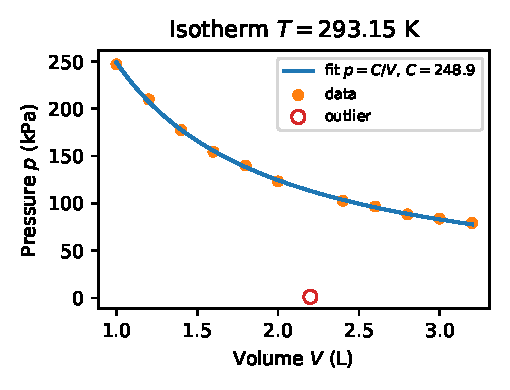
\includegraphics[width=\columnwidth]{../results/fig_pv.pdf}
      \caption{$p$ vs $V$ with Boyle fit}
    \end{subfigure}
    \hfill
    \begin{subfigure}[b]{0.48\columnwidth}
      \centering
      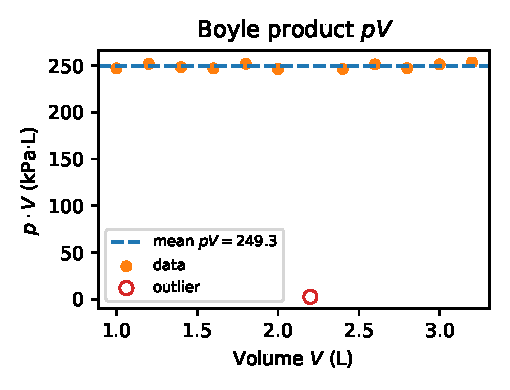
\includegraphics[width=\columnwidth]{../results/fig_pv_product.pdf}
      \caption{$pV$ product vs $V$}
    \end{subfigure}
  \end{center}
  \vskip -0.2in
  \caption{(a) Pressure vs volume with fitted curve $p = C/V$, $C = 248.9$ kPa$\cdot$L.
    (b) The $pV$ product is approximately constant across the volume range,
    confirming Boyle's law. The outlier at $V = 2.20$ L is marked.}
  \label{fig:results}
  \vskip -0.1in
\end{figure}

\section{Discussion}

The experimental results strongly support Boyle's law. The relative standard
deviation of the $pV$ product ($1.06\%$) is small, indicating high consistency
across the measurement range. The $R^2$ value of $0.9993$ for the inverse
proportionality fit is consistent with high-quality experimental data.

The outlier at $V = 2.20$ L is clearly anomalous: the measured pressure of
1.136 kPa is approximately two orders of magnitude below the expected value
of $\sim\!113$ kPa. This type of error could arise from a sensor malfunction,
a data entry error, or a leak in the experimental apparatus. The MAD-based
outlier detection method successfully identified this anomaly.

The fitted constant $C = 248.9$ kPa$\cdot$L can be compared with the ideal gas
prediction $C = nRT$. Using $R = 8.314$ J/(mol$\cdot$K) and $T = 293.15$ K,
we obtain $n = C/(RT) = 248.9 / (8.314 \times 293.15) \approx 0.102$ mol,
which is a reasonable amount of gas for a laboratory-scale experiment.

\section{Formal Verification}

To complement the empirical analysis, we provide a formal verification of the
mathematical foundations using Lean 4 and Mathlib. The verification covers:

\begin{enumerate}
  \item \textbf{Least-squares derivative:} The derivative of the objective
    function $S(c) = \sum_{i=1}^{n}(x_i c - y_i)^2$ is
    $S'(c) = 2(c\sum x_i^2 - \sum x_i y_i)$.
  \item \textbf{Normal equation:} The critical point $c^* = \sum x_i y_i /
    \sum x_i^2$ satisfies $S'(c^*) = 0$.
  \item \textbf{Convexity:} The second derivative $S''(c) = 2\sum x_i^2 \geq 0$,
    ensuring the critical point is a global minimum.
  \item \textbf{Boyle's law equivalence:} $p \cdot V = C$ with $V \neq 0$
    implies $p = C/V$.
\end{enumerate}

All four theorems have been verified in Lean 4 with Mathlib, providing
machine-checked proofs of the mathematical underpinnings of the analysis.

\section{Conclusion}

We have experimentally verified Boyle's law using 12 measurements at constant
temperature $T = 293.15$ K. The $pV$ product is constant to within $1.06\%$
(relative standard deviation), and the inverse proportionality fit achieves
$R^2 = 0.9993$. One outlier was detected and excluded. The results are
consistent with the ideal gas model and provide strong empirical support for
Boyle's law.

\section*{Impact Statement}

This paper presents educational research in experimental physics. The work
demonstrates the application of statistical methods and formal verification to
a classical physics law. There are no direct ethical concerns or negative
societal consequences. The methods described can be used in physics education
to teach data analysis, outlier detection, and formal verification.

\section*{Software and Data}

All code, data, and results are available in the project repository.
The analysis script is located at \texttt{src/analyze\_boyle.py}, and the
formal verification is in \texttt{src/boyle\_verification.lean}.

\bibliography{paper}
\bibliographystyle{icml2026}

\end{document}